\documentclass[a4paper]{article}

\usepackage[utf8]{inputenc}
\usepackage[serbian]{babel}

\usepackage{tikz}
\usepackage{tcolorbox}
\usepackage{amsmath}
\usepackage{amsthm}
\usepackage{nameref}
\usepackage{listings}
\usepackage{fancyhdr}

\makeatletter
\newcommand*{\currentname}{\@currentlabelname}
\makeatother

\begin{document}
    \begin{titlepage}
    \begin{tabular}{ l  c   r  }
        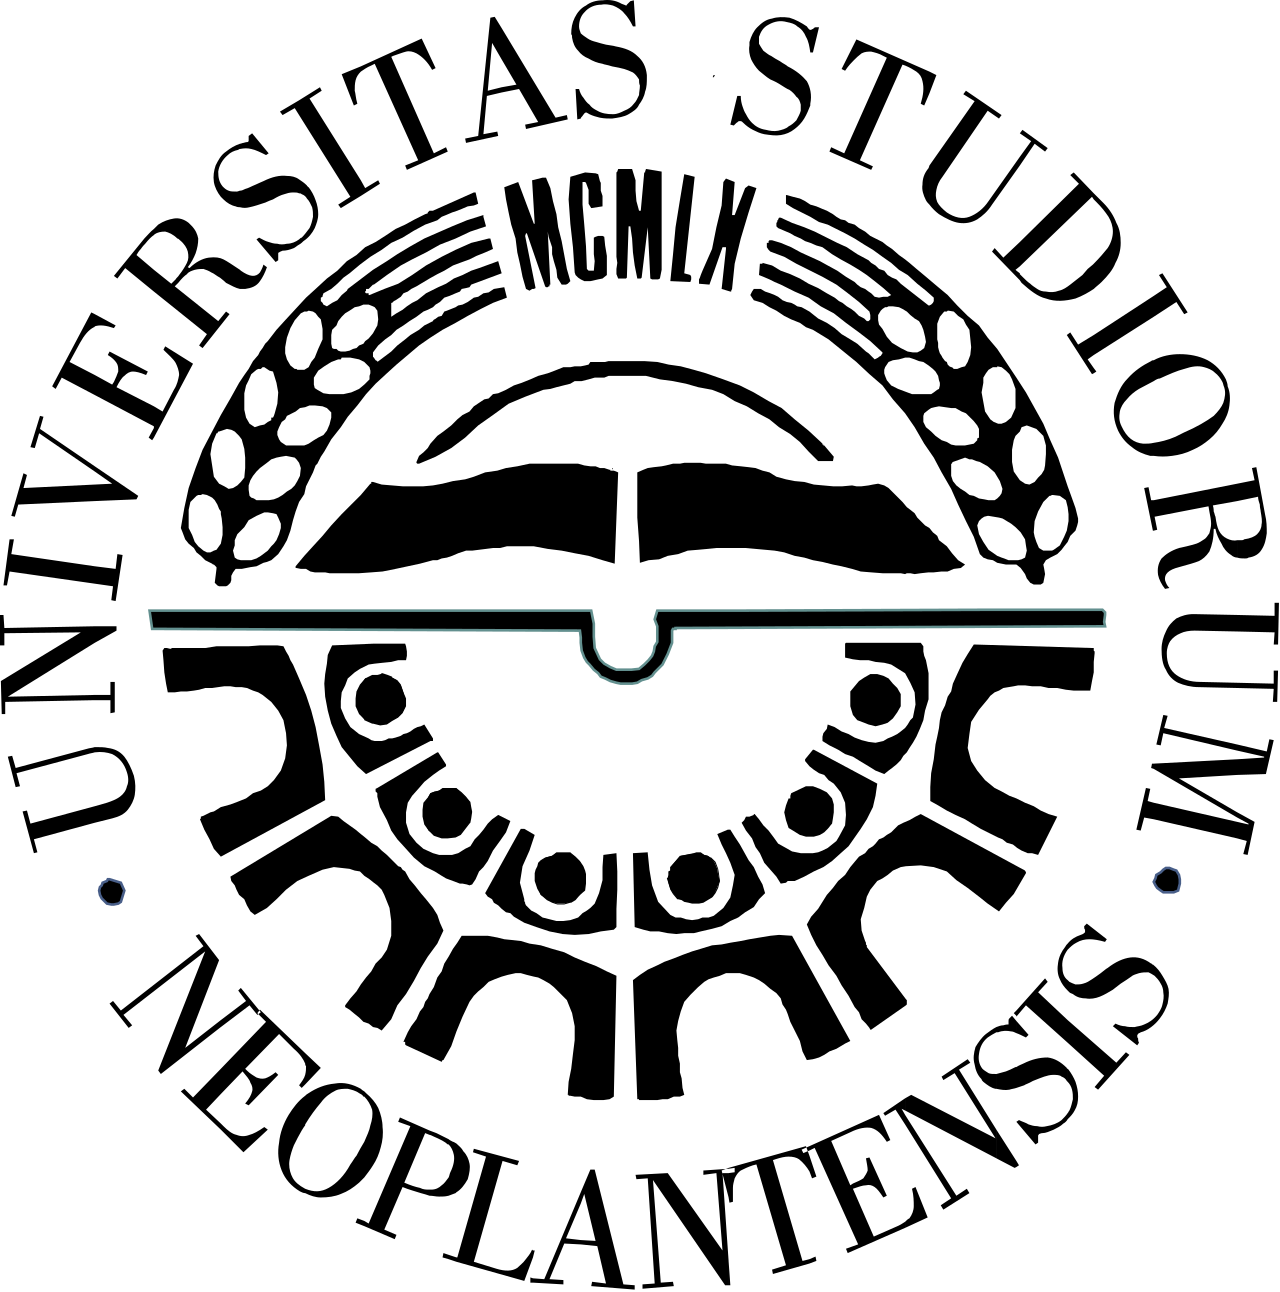
\includegraphics[height=0.1\textwidth, width=0.1\textwidth]{img/uns.png} &
        \begin{tabular}{c}
            \large\textbf{UNIVERZITET U NOVOM SADU} \\
            \large\textbf{FAKULTET TEHNIČKIH NAUKA}  \\
        \end{tabular}
        
\includegraphics[height=0.1\textwidth, width=0.1\textwidth]{img/ftn-logo.jpg}
    \end{tabular}
    \vspace*{1cm}
    \begin{flushleft}
        UNIVERZITET U NOVOM SADU \\
        FAKULTET TEHNIČKIH NAUKA \\
        NOVI SAD \\
        Departman za računarstvo i automatiku \\
        Odsek za računarsku tehniku i računarske komunikacije \\
    \end{flushleft}
    \vspace*{2cm}
    \begin{center}
        \LARGE\textbf{ISPITNI RAD}
    \end{center}
    \vspace*{0.25cm}
    \begin{flushleft}
        \begin{tabular}{l l}
            Kandidat:& Lazar Nagulov \\
            Broj indeksa:& SV61/2022 \\
            & \\
            Predmet:&    Objektno orijentisano programiranje 2 \\
            Tema rada:&	Sudoku \\
            & \\
            & \\
            Mentor rada:&    dr Miodrag Đukić
        \end{tabular}
    \end{flushleft}
    \vfill
    \begin{center}
        Novi Sad, decembar, 2023.
    \end{center}
\end{titlepage}
    \pagestyle{fancy}
    
\rhead{SADRŽAJ}
\lhead{}
\pagenumbering{Roman}
\tableofcontents
\newpage

\rhead{SPISAK SLIKA}
\listoffigures
\newpage

\rhead{SPISAK TABELA}
\listoftables
\newpage
    
    \section{Uvod}
    \pagenumbering{arabic}
    \rhead{1. Uvod}
    \subsection{Sudoku}
    Sudoku je logička zagonetka najčešće u obliku $9 \times 9$ tabele (matrice).
    U prazna polja tabele se upisuju cifre, tako da se svaka broj mora pojaviti
    tačno jednom u svakom redu, svakoj koloni i svakoj $3\times 3$ podmatrici (bloku).
    \begin{figure}[h]
        \centering
        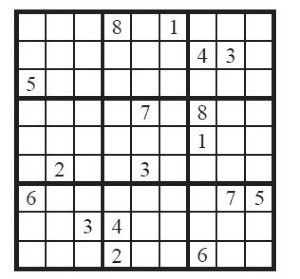
\includegraphics[width=0.5\textwidth, height=0.5\textwidth]{img/sudoku-example.jpg}
        \caption{Primer sudoku zagonetke}
    \end{figure}
    \par Zagonetka ne mora da ima jedno rešenje, ali je standard da ga ima. Primer rešenje zagonetke sa slike 1:
    \begin{figure}[h]
        \centering
        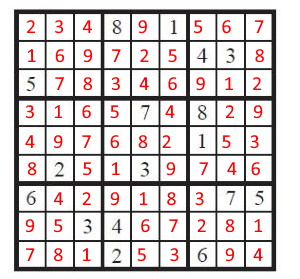
\includegraphics[width=0.5\textwidth, height=0.5\textwidth]{img/sudoku-example-sol.jpg}
        \caption{Primer rešenja sudoku zagonetke}
    \end{figure}
    
    \subsection{Zadatak}
    Realizovati konzolnu aplikaciju koja omogućava rešavanje i generisanje sudoku zagonetki. Korisnik unosi dateteke kroz argumente komandne linije. 
    Primer pokretanja programa:
    \par\texttt{./sudoku $input.txt$ $output.txt$}\\
    Argumenti:
    \begin{enumerate}
        \item $input.txt$ - Datoteka iz koje se čita zagonetka.
        \item $output.txt$ - Datoteka u koju se upisuje zagonetka.
    \end{enumerate}
    \par Nakon pokretanja programa, korisniku se prikazuje početni meni koji nudi opcije:
    \begin{itemize}
        \item \texttt{Generate new Sudoku puzzle} - Generisanja nove zagonetke.
        \item \texttt{Load Sudoku puzzle from file} - Učitavanja zagonetke.
        \item \texttt{Exit} - Izlaska iz igre.
    \end{itemize}
    Nakon generisanja ili učitavanja zagonetke, korisnik može da:
    \begin{itemize}
        \item \texttt{Import solution} - Učita rešenje.
        \item \texttt{Solve} - Dopusti programu da reši zagonetku.
        \item \texttt{Exit} - Izlađe iz igre.
    \end{itemize}
    \par Na konzolnoj aplikaciji, posle rešavanja koje je generisao program ili učitao iz datoteke, prikazuju se statistički podaci igre, uključujući broj dobro 
    postavljenih polja, broj grešaka i brojač odigranih igara i spisak svih pronađenih grešaka. Nakon završetka igre, korisnik ima opciju da odabere ponovno igranje, 
    što pokreće novu iteraciju igre.
    \newpage

    \rhead{2. Analiza problema}
    \section{Analiza problema}
    \newpage

    \rhead{3. Koncept rešenja}
    \section{Koncept rešenja}
    
    \subsection{Algoritmi za rešavanje zagonetke}
    \subsubsection{Obrnuta pretraga}
    Najtrivijalniji algoritam za rešavanje sudoku zagonetke je obrnuta pretraga (eng. Backtracking).
    Ovo je algoritam grube sile (eng. Brute force) koji isprobava sve moguće kombinacije. Dakle, potrebno je da se prođe kroz
    svako polje u tabeli. Ukoliko je polje prazno, upisujemo cifru koja u trenutnoj tabeli ispunjava sva pravila. Nakon upisivanje cifre, rekurzivno pozivamo funkciju 
    - pokušavamo da pronađe rešenje sa novom tabelom. Ukoliko rešenje nije pronađeno, vraćamo se nazad i upisujemo drugu cifru. 
    \par Vremenska složenost ovog algoritma je $\mathcal{O}(n ^ m)$, gde je $n$ dimenzija tabele, a $m$ broj polja koja trebaju da se popune.
    (U našem slučaju je složenost $\mathcal{O}(9^n)$). Minimalan broj polja koja
    moraju biti popunjena je $17$, dakle, u najgorem slučaju se provera $9^{64}$ mogućnosti!
    
    \subsubsection{Optimizacija obrnute pretrage}
    Način na koji možemo optimizovati algoritam obrnute pretrage je da ubrzamo proveru da li se broj može postaviti na zadatoj poziciji. To ćemo postići tako što ćemo pamtiti
    koji broj se našao u redu, koloni i bloku. Za to ćemo koristiti \texttt{std::bitset<>} iz zaglavlja \texttt{bitset} gde, ako se za $i \in [0,8]$ na $i$-toj poziciji nalazi 1, znači da se cifra $i+1$ nalazi u redu, koloni ili bloku.
    \par Pre samog ulaska u rekurzivnu funkciju obrnute pretrage, moramo proći kroz tabelu i zapisati svaki broj koji se nalazi u tabeli u nizove bitova. Potrebna su 3 niza bitova - 
    \begin{figure}[h]
        \centering
        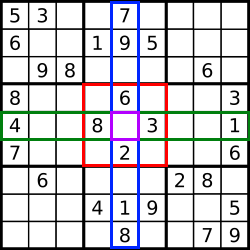
\includegraphics[width=0.5\textwidth, height=0.5\textwidth]{img/conversion.png}\\
        \texttt{Polje (4,4)}\\
        \begin{tabular}{ l r }
            \texttt{RowSet: } & \texttt{010001101}\\
            \texttt{ColSet: } & \texttt{111100011}\\
            \texttt{BlockSet:}& \texttt{010100110}\\
        \end{tabular}
        \caption{Primer konverzije polja u binaran broj}
    \end{figure}
    za red, kolonu i blok. Za proveru da li je cifru moguće upisati
    koristimo bitnu operaciju ili (eng. bitwise or): 
    \par\texttt{std::bitset<> contain = rows[row] | cols[col] | blocks[block];}\\
    Novi niz bitova \texttt{contain} ima $0$ na $i$-toj poziciji ako je moguće postaviti cifru $i+1$ na poziciju '(row, col)'. Na slici 3 vidimo da se u 
    redu nalaze brojevi 1,3,4,8 (010001101), koloni 7,9,6,2,1,8 (111100011) i u bloku 6,3,2,8 (010100110). Iz ovoga zaključujemo da je u polje (4,4)
    moguće upisati broj 5 (111101111).
    \par Vremenska složenost je i dalje $\mathcal{O}(n^m)$, gde je $n$ dimenzija tabele, a $m$ broj polja koja trebaju da se popune, stim da je su sve provere da li se broj može upisati 
    u polje svedene na $\mathcal{O}(m)$ za razliku od prethodnog algoritma koji ima složenost $\mathcal{O}(nm)$.
    \begin{table}[h]
        \centering
        \begin{tabular}{ |c|c|c|c|}
            \hline
            & Maksimum & Medijana & Srednja vrednost \\
            \hline
            Gruba sila & 6.20147s & 0.001222s & 0.04691s \\
            \hline
            Optimizacija & 2.14567s & 0.00072s & 0.02301s \\
            \hline
        \end{tabular}
        \caption[Optimizacija obrnute pretrage]{Optimizacija obrnute pretrage - 1000 zagonetaka sa 25 popunjenih polja.}
    \end{table}

    \subsection{Algoritmi za generisanje zagonetke}
    \subsubsection{Koraci u generisanju zagonetke}
    Generisanje zagonetke se može opisati u dva koraka:
    \begin{enumerate}
        \item Popuniti čitavu tabelu slučajnim vrednostima [1, \texttt{BOARD\_SIZE}].
        \item Nasumično obrisati brojeve iz tabele.
    \end{enumerate}
    \par Primetimo da se blokovi na glavnoj dijagonali mogu zasebno popuniti jer ne utiču jedan na drugog. Dakle, prvi korak u generisanju se svodi na 
    popunjavanja glavne dijagonale i rešavanja tako generisane zagonetke. Zatim brišemo brojeve iz tabele. Koliko brojava trebamo obrisati zavisi od težine zagonetke
    koju želimo generisati (Tabela 2).
    \begin{table}[h]
        \centering
        \begin{tabular}{ | c | c |}
            \hline
            Težina & Broj popunjenih polja \\
            \hline
            Lako & 32 - 38\\
            \hline
            Srednje & 26 - 31\\
            \hline
            Teško & 22 - 25\\
            \hline
            Veoma teško & 17 - 21\\
            \hline
        \end{tabular}
        \caption{Težina zagonetke u odnosu na broj popunjenih polja}
    \end{table}
    \subsubsection{Generisanje pseudoslučajnih brojeva}
    \newpage
    
    \rhead{4. Opis rešenja}
    \section{Opis rešenja}
    
    \subsection{Modul glavnog programa}
    \texttt{int main(int argc, char** argv);}
    \par Glavna funckija programa.

    \subsection{Modul Sudoku}
    
    \subsubsection{Članovi}
    \begin{tabular}{ l l }
        \texttt{int currentRound;} & Trenutna runda\\
        \texttt{int correctCount;} & Broj tačnih cifara\\
        \texttt{int wrongCount;} & Broj pogrešnih cifara\\
        \texttt{Board board;} & Sudoku tabela\\
    \end{tabular}
    
    \subsubsection{Enumeracije}
    \texttt{enum Difficulty;}
    \par Određuje težinu Sudoku zagonetke na osnovu broja izbrisanih polja. \\ 
    Vrednost: \texttt{EASY, MEDIUM, HARD, VERY\_HARD}

    \subsubsection{Funkcija članica za pokretanje (Run)}
    \texttt{void Run();}
    \par Pokreće aplikaciju i kreira početni meni za korisnika. Nudi korisniku mogućnost da generiše ili učita zagonetku iz datoteke. 
    U njoj se nalazi glavna petlja igre.

    \subsubsection{Funcija članica za unos rešenja (SolvingOptions)}
    \texttt{void SolvingOptions();}
    \par Nudi korisniku mogućnost da učita rešenje ili da dopusti programu da sam reši zagonetku. Poziva se  iz \texttt{Run()} funkcije nakon generisanja 
    ili učitavanja zagonetke.

    \subsubsection{Funkcija članica za rešavanje zagonetke (Solve)}
    \texttt{void Solve();}
    \par Rešava zagonetku koristeći algoritam obrnute pretrage.

    \subsubsection{Funckija članica za proveru rešenja (Check solution)}
    \texttt{void CheckSolution(std::ifstream\& in);}
    \par Učitava zagonetku iz datoteke i proverava da li je validna. Ispisuje sve greške koje pronađe, njihov broj i broj tačno upisanih brojeva.\\
    Parametri:
    \begin{itemize}
        \item (\texttt{std::ifstream\&}) in - datoteka iz koje se čita rešenje.
    \end{itemize}

    \subsubsection{Funkcija članica za gerenisanje zagonetke (Generate)}
    \text{void Generate(Difficulty difficulty);}
    \par Generiše Sudoku zagonetku sa zadatom težinom. \\
    Parametri:
    \begin{itemize}
        \item (\texttt{Sudoku::Difficulty}) difficulty - enumeracija koja označava težinu zagonetke.
    \end{itemize}
   
   
    \subsection{Modul Tabela}
    
    \subsubsection{Konstante}
    \begin{tabular}{ l l }
        \par\texttt{int BOARD\_SIZE = 9;} & Veličina tabele. \\
        \par\texttt{int BLOCK\_SIZE = 3;} & Veličina bloka. \\
        \par\texttt{int EMPTY = 0;}  & Oznaka za prazno polje. \\
        \par\texttt{char EMPTY\_CHAR = '\_';}  & Oznaka za prazno polje prilikom ispisa.
    \end{tabular}
    
    \subsubsection{Članovi}
    \begin{tabular}{ l l }
        \par\texttt{int board[BOARD\_SIZE * BOARD\_SIZE];} & Niz koji predstavlja tabelu.\\
    \end{tabular}

    \subsubsection{Alijas BitArray}
    {\parindent0pt
    \texttt{using BitArray = }\\
    \texttt{std::array<std::bitset<Board::BOARD\_SIZE>, Board::BOARD\_SIZE>;}
    }
    \par Niz od \texttt{Board::BOARD\_SIZE} setova bitova dužine \texttt{Board::BOARD\_SIZE}.
    
    \subsubsection{Funkcija članica za proveru poteza (IsPossibleMove)}
    \texttt{bool IsPossibleMove(int row, int col, int number) const;}
    \par Proverava da li je moguće postaviti broj 'number' na poziciju '(row, col)'.\\
    Parametri:
    \begin{itemize}
        \item (\texttt{int}) row - red u tabeli
        \item (\texttt{int}) col - kolona u tabeli
        \item (\texttt{int}) number - broj koji se pokušava staviti
    \end{itemize}
    Povratna vrednost:
    \begin{itemize}
        \item (\texttt{bool}) - true ako je moguće postaviti broj, false ako nije.
    \end{itemize}

    \subsubsection{Funckija članica za proveru validnosti tabele (IsValid)}
    \texttt{bool IsValid() const;}
    \par Proverava da li trenutna tabela ispunjava sva pravila sudoka.
    
    \subsubsection{Funkcija članica za pronalaženje grešaka (CountErrors)}
    \texttt{int CountErrors(const Board\& original) const;}
    \par Prebrojava i ispisuje sve greške u tabeli.\\
    Povratna vrednost:
    \begin{itemize}
        \item (\texttt{int}) Broj grešaka u tabeli.
    \end{itemize}

    \subsubsection{Funkcija članica za dobavljanje elementa tabele (At)}
    \texttt{int\& At(int row, int col);}
    \par Dobavlja element na poziciji '(row, col)'. Proverava granice.
    
    \subsubsection{Statična funkcija članica za dobavljanja blocka (GetBlock)}
    \texttt{static constexpr int GetBlock(int row, int col);}
    \par Vraća blok u kome se nalazi polje '(row, col)'.\\
    Parametri:
    \begin{itemize}
        \item (\texttt{int}) row - Red u tabeli.
        \item (\texttt{int}) col - Kolona u tabeli.
    \end{itemize}
    Povratna vrednost:
    \begin{itemize}
        \item (\texttt{int}) Broj bloka u kome se nalazi polje (row, col)
    \end{itemize}

    \subsubsection{Funkcija članica za generisanje elemenata na glavnoj dijagonali (GenerateDiagonal)}
	\texttt{void GenerateDiagonal();}
	\par Generiše nasumično elemente na glavnoj dijagonali.

    \subsubsection{Funcija članica za generisanje ostalih elemenata (GenerateOther)}
    \texttt{bool GenerateOther(int row, int col);}
    \par Rekurzivno generiše nasumično elemente koji se ne nalaze na glavnoj dijagonali.\\
	Parametri:
    \begin{itemize}
        \item (\texttt{int}) row - Početan red (uglavnom 0).
        \item (\texttt{int}) col - Početna kolona (uglavnom 0).
    \end{itemize}
    Povratna vrednost:
    \begin{itemize}
        \item (\texttt{bool}) Zaustavlja rekurzivno generisanje tabele.
    \end{itemize}
    
    \subsubsection{Funkcija članica za popunjavanje blokova (FillBlock)}
    \texttt{void FillBlock(int row, int col);}
    \par Rekurzivno generiše nasumično elemente u bloku.\\
    Parametri:
    \begin{itemize}
        \item (\texttt{int}) row - početni red (gornje levo polje u bloku).
        \item (\texttt{int}) col - početna kolona (gornje levo polje u bloku).
    \end{itemize}

    \subsubsection{Funkcija članica za brisanje elemenata iz tabele (RemoveNumber)}
	\texttt{void RemoveNumber(int count);}
    \par Nasumično briše $count$ elementa iz tabele.\\
    Parametri:
    \begin{itemize}
        \item (\texttt{int}) count - broj elemenate koliko se briše iz tabele.
    \end{itemize}

    \subsubsection{Funkcija članica koja implementira algoritam obrnute pretrage (Backtrack)}
    {\parindent0pt
    \texttt{bool Backtrack(BitArray\& rSet, BitArray\& cSet, BitArray\& bSet);}
    }
    \par Funkcija implementira algoritam obrnute pretrage. Rekurzivno popunjava tabelu. Poziva se iz funkcije \texttt{Solve()} nakon generisanja pomoćnih nizova bitova.
    Parametri:
    \begin{itemize}
        \item (\texttt{BitArray}) rSet - Pomoćni niz koji prati pojavljivanje brojeva u redovima.
        \item (\texttt{BitArray}) cSet - Pomoćni niz koji prati pojavljivanje brojeva u kolonama.
        \item (\texttt{BitArray}) bSet - Pomoćni niz koji prati pojavljivanje brojeva u blokovima.
    \end{itemize}
    Povratna vrednost:
    \begin{itemize}
        \item (\texttt{bool}) Zaustavlja rekurziju kada pronađe rešenje.
    \end{itemize}

    \subsubsection{Funkcija članica za pronalaženje prvog praznog polja (FindEmpty)}
	\texttt{bool FindEmpty(int\& row, int\& col);}
    \par Pronalazi prvo prazno polje od pozicije '(row, col)'. Prazno polje se nalazi u $row$ i $col$ promenljivi nakon završetka funkcije.\\
    Parametri:
    \begin{itemize}
        \item (\texttt{int\&}) row - referenca na početan red koji se pretražuje.
        \item (\texttt{int\&}) col - referenca na početnu kolonu koja se pretražuje.
    \end{itemize}

    \subsubsection{Funckija članica za brisanje tabele (Clear)}
    \texttt{void Clear();}
    \par Postavlja sve elemente u tabeli na 0.

    \subsubsection{Operatori upisa i ispisa}
    \par\texttt{std::istream\& operator>>(std::istream\& in, Board\& b);}
    \par\texttt{std::ostream\& operator<<(std::ostream\& out, const Board\& b);}
    \par\texttt{std::ofstream\& operator<<(std::ofstream\& out, const Board\& b);}
    
    \subsubsection{Operator dobavljanja}
    \par\texttt{int\& operator()(int row, int col);}
    
    
    
    \section{Testiranje}
    \newpage
    \section{Uočeni problemi i ograničenja}
    \newpage
    \section{Zaključak}
    \newpage
\end{document}